% =============================================================================
% P3D -- Privacy 2: poster (EN)
% Format: A3 portrait (297 x 420 mm), ONE page, two columns, Latin Modern.
% Expected figures in out/: FigP1_EN.pdf, Fig5_EN.pdf (compiled from figuras/).
% The heat map (Figure P2) is a colored table written in this file.
% Content mirrors MD/P3D_Privacidade2_Poster_EN.md.
%
% ONE PAGE: all content sits inside a single box (\parbox) wrapped by adjustbox with
% "max totalsize": if the content is taller than the page it is scaled down
% proportionally until it fits; if it is shorter it is not enlarged.
% Size tuning: \corpo (text size). Authors: edit the \blocoautores block.
% =============================================================================
\documentclass[12pt]{article}

\usepackage[T1]{fontenc}
\usepackage[utf8]{inputenc}
\usepackage{lmodern}
\usepackage[paperwidth=297mm,paperheight=420mm,margin=10mm]{geometry}
\usepackage[brazil,english]{babel}
\usepackage{graphicx}
\usepackage{xcolor}
\usepackage{array}
\usepackage{colortbl}
\usepackage[skins]{tcolorbox}
\usepackage{adjustbox}
\usepackage[expansion=false]{microtype}

\pagestyle{empty}
\setlength{\parindent}{0pt}
\setlength{\parskip}{0pt}

\definecolor{exLine}{RGB}{23,54,93}
\definecolor{exFill}{RGB}{220,233,247}
\definecolor{prFill}{RGB}{200,240,236}
\definecolor{prLine}{RGB}{8,127,140}
\definecolor{prText}{RGB}{6,79,87}
\definecolor{ctxText}{RGB}{38,52,67}

\newcommand{\corpo}{\fontsize{14}{18}\selectfont}
\newcommand{\figtitulo}[1]{{\fontsize{17}{21}\selectfont\bfseries\color{exLine}#1\par}\vspace{2mm}}
\newcommand{\leitura}[1]{\vspace{2mm}{\corpo\itshape\color{ctxText}#1\par}}

% --- Authors, course and code (edit here) -----------------------------------
\newcommand{\blocoautores}{%
  \textbf{Authors:} Filipe Alves de Sousa and members of the Colégio Reciclagem 1 group\\
  \textbf{Course:} IT Project Management (GPTI) -- PPCA/CIC/UnB\\
  \textbf{Code:} 3p2 / 3R31}

\newtcolorbox{caixa}[1]{enhanced,colback=white,colframe=exLine,boxrule=0.7mm,arc=2mm,
  left=4mm,right=4mm,top=3mm,bottom=3.5mm,
  title={#1},fonttitle=\fontsize{17}{21}\selectfont\bfseries,coltitle=white,colbacktitle=exLine}

\begin{document}
\thispagestyle{empty}
\corpo

\noindent\begin{adjustbox}{max totalsize={\textwidth}{\textheight},center}
\parbox{\textwidth}{%

% ------------------------------- BANNER --------------------------------------
\begin{tcolorbox}[enhanced,colback=exLine,colframe=exLine,coltext=white,arc=2mm,
  left=6mm,right=6mm,top=4.5mm,bottom=4.5mm]
{\fontsize{30}{34}\selectfont\bfseries PMBOK 8 on one page: principles, processes and tailoring\par}
\vspace{2.5mm}
{\fontsize{15}{19}\selectfont SIPA Privacy 2 group \ $\cdot$ \ PMBOK 8 summary\par}
{\fontsize{15}{19}\selectfont\bfseries Central idea: principles guide decisions; domains and Focus Areas help locate the work; tailoring adjusts how it is carried out [5].\par}
\vspace{2.5mm}
{\fontsize{14}{18}\selectfont\blocoautores\par}
\end{tcolorbox}

\vspace{4mm}

\noindent
\begin{minipage}[t]{0.485\linewidth}
% ------------------------------ LEFT COLUMN ----------------------------------
\figtitulo{Figure P1 --- How the pieces relate}
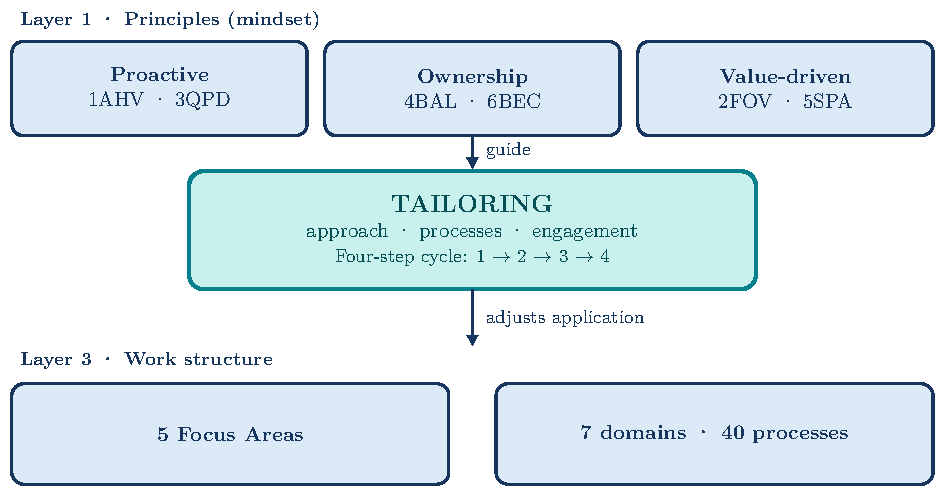
\includegraphics[width=\linewidth]{out/FigP1_EN.pdf}
\leitura{\textbf{Five operations on processes:} add $\cdot$ modify $\cdot$ remove $\cdot$ blend $\cdot$ align. \textbf{Three objects of tailoring:} life cycle and development approach $\cdot$ processes $\cdot$ engagement [5].}

\vspace{4mm}

\figtitulo{Figure P3 --- Four concentrations for reading the seven domains}
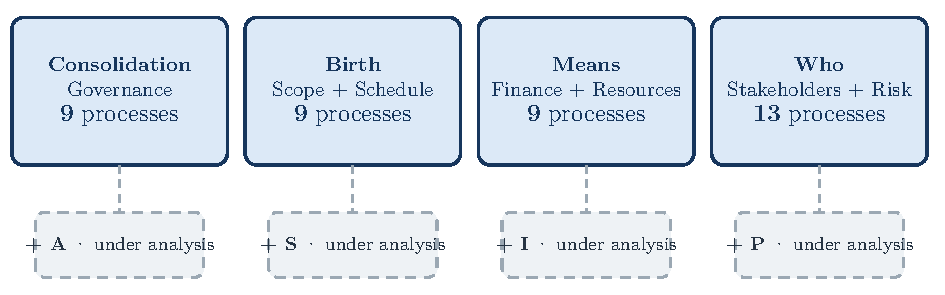
\includegraphics[width=\linewidth]{out/Fig5_EN.pdf}
\leitura{\textbf{Reading notice:} the four concentrations and the A, S, I, and P labels are the \textbf{analytical grouping of this work}; the seven domains and their 40 processes are from PMBOK 8 [5].}
\end{minipage}\hfill
\begin{minipage}[t]{0.485\linewidth}
% ------------------------------ RIGHT COLUMN ---------------------------------
\figtitulo{Figure P2 --- 40 processes in 7 domains $\times$ 5 Focus Areas}
{\fontsize{15}{20}\selectfont
\renewcommand{\arraystretch}{1.35}
\noindent\begin{tabular*}{\linewidth}{@{\extracolsep{\fill}}lrrrrrr}
\hline
\textbf{Domain} & \textbf{IN} & \textbf{PL} & \textbf{EX} & \textbf{MC} & \textbf{CL} & \textbf{Total}\\
\hline
Governance & \cellcolor{exLine!9}1 & \cellcolor{exLine!18}2 & \cellcolor{exLine!27}3 & \cellcolor{exLine!18}2 & \cellcolor{exLine!9}1 & 9\\
Scope & 0 & \cellcolor{exLine!36}4 & 0 & \cellcolor{exLine!18}2 & 0 & 6\\
Schedule & 0 & \cellcolor{exLine!18}2 & 0 & \cellcolor{exLine!9}1 & 0 & 3\\
Finance & 0 & \cellcolor{exLine!27}3 & 0 & \cellcolor{exLine!9}1 & 0 & 4\\
Stakeholders & \cellcolor{exLine!9}1 & \cellcolor{exLine!18}2 & \cellcolor{exLine!18}2 & \cellcolor{exLine!18}2 & 0 & 7\\
Resources & 0 & \cellcolor{exLine!18}2 & \cellcolor{exLine!18}2 & \cellcolor{exLine!9}1 & 0 & 5\\
Risk & 0 & \cellcolor{exLine!36}4 & \cellcolor{exLine!9}1 & \cellcolor{exLine!9}1 & 0 & 6\\
\hline
\textbf{Total} & \textbf{2} & \textbf{19} & \textbf{8} & \textbf{10} & \textbf{1} & \textbf{40}\\
\hline
\end{tabular*}\par}
\leitura{\textbf{Legend:} IN Initiating $\cdot$ PL Planning $\cdot$ EX Executing $\cdot$ MC Monitoring and Controlling $\cdot$ CL Closing. Process count $\neq$ duration or importance of an area. \textit{Identify Stakeholders} is in Initiating (Guide Figure 2-32).}

\vspace{4mm}

\begin{caixa}{In practice and limits}
\corpo
PMBOK 8 does not mention digital twins. Hybrid approaches are frequent in practice [4, 6]; tailoring is therefore the axis of this summary.
\end{caixa}

\vspace{4mm}

\begin{caixa}{Key references}
\fontsize{11}{14}\selectfont
Numbering of the full report.\par\smallskip
[4] NOLL, J.; BEECHAM, S. How agile is hybrid agile? An analysis of the HELENA data. \textbf{Product-Focused Software Process Improvement (PROFES 2019)}, LNCS vol. 11915, pp. 341-349, 2019.\par\smallskip
[5] PMI. \textbf{The Standard for Project Management and A Guide to the PMBOK (PMBOK Guide)}. 8th ed., 2025. Restricted-access document.\par\smallskip
[6] REED, A. H. et al. Usage of hybrid project management approaches and influences on approach selection. \textbf{Communications of the Association for Information Systems}, vol. 54, 2024.
\end{caixa}
\end{minipage}

}% end of \parbox
\end{adjustbox}

\end{document}
